% ---------------------------------------------------- %
% Budburst 2015 manuscript
% Preamble
% ---------------------------------------------------- %
\documentclass[11pt]{article}
\renewcommand{\baselinestretch}{1.8}
\usepackage{textcomp}
\usepackage{fontenc}
\usepackage{graphicx}
\usepackage{caption} % for Fig. captions
\usepackage{gensymb} % for \degree
\usepackage{placeins} % for \images
\usepackage[margin=1in]{geometry} % to set margins
\usepackage{setspace}
\usepackage{lineno}
\usepackage{cite}
\usepackage{amssymb} % for math symbols
\usepackage{amsmath} % for aligning equations
\usepackage{natbib}

% \setlength{\parindent}{0pt}

% \renewcommand{\familydefault}{\sfdefault} % for nicer sans serif font
\graphicspath{{images/}}	% Root directory of the Fig.s
% \setlength{\parskip}{1 mm}


%\usepackage{Sweave}
\begin{document}
 
  
\noindent \textbf{\large{Temperature and photoperiod drive spring phenology across all species in a temperate forest community}}


\noindent Brief heading: Phenological cues and community assembly\\ 

\noindent Authors:\\
D. F. B. Flynn$^{1,2\dagger}$ \& E. M. Wolkovich$^{1,2\dagger *}$
\vspace{2ex}\\
\emph{Author affiliations:}\\
$^{1}$Arnold Arboretum of Harvard University, 1300 Centre Street, Boston, Massachusetts, 02130, USA; \\
$^{2}$Organismic \& Evolutionary Biology, Harvard University, 26 Oxford Street, Cambridge, Massachusetts, 02138, USA
\vspace{2ex}\\
$^*$Corresponding author: 604.827.5246; e.wolkovich@ubc.ca\\
$^\dagger$Authors contributed equally\\

\noindent \emph{Keywords:} climate change, forcing temperatures, chilling, temporal niche, daylength, winter temperatures, forest communities\\ % 5-8 New Phyto says we should include title words
\emph{Paper type:} Full paper\\
 \emph{Counts}: Total word count for the main body of the text:  5022; Introduction: 1065; M \& M: 966; Results: 715; Discussion: 2276; 3 figures (all in color). Supporting Information of notes, 7 supplemental tables and 9 supplemental figures.\\


%%%%%%%%%%%%%%%%%%%%%%%%%%%%%%%%%%%%
% Abstract
%%%%%%%%%%%%%%%%%%%%%%%%%%%%%%%%%%%%

\newpage % 200/200 (if they don't count the #s)
\noindent {\bf Summary:}\\
(1) Accurate predictions of spring plant phenology with climate change are critical for projections of growing seasons, plant communities and a number of ecosystem services, including carbon storage. Progress towards prediction, however, has been slow because the major cues known to drive phenology---temperature (including  winter chilling and spring forcing) and photoperiod---generally covary in nature and may interact, making accurate predictions of plant responses to climate change complex and non-linear. Alternatively, recent work suggests many species may be dominated by one cue, which would make predictions much simpler. \\
(2) We manipulated all three cues across 28 woody species from two North American forests.\\
(3) All species responded to all cues examined. Chilling exerted a strong effect, especially on budburst (-15.8 days), with responses to forcing and photoperiod greatest for leafout (-19.1 and -11.2 days, respectively). Interactions between chilling and forcing suggest each cue may compensate somewhat for the other. Cues varied across species, leading to staggered leafout within each community and supporting the idea that phenology is a critical aspect of species' temporal niches. \\
(4) Our results suggest that predicting the spring phenology of communities will be difficult, as all species we studied could have complex, non-linear responses to future warming. 

\newpage
% \linenumbers
%%%%%%%%%%%%%%%%%%%%%%%%%%%%%%%%%%%%
% Main text is ~2300 ... methods is about 750 ... these counts all include extended citation format. 

Plant phenology---the timing of recurring life history events, such as leafout and flowering---is critical to the structure and function of ecosystems \citep{Cleland:2007aa}. Spring plant phenology in particular drives local ecosystem properties, from the length of the growing season to energy balance between land and atmosphere, and scales up to impact global carbon cycles \citep{Richardson:2009aa}. % Plant phenology determines the timing of the basal resource in most systems, and thus shapes food webs and mutualistic networks

Phenology is also one of the major biological indicators of climate change, with plant phenology shifting earlier across the globe 4-6 days/\degree C with warming \citep{IPCC:2014sm}. While this average response is strikingly consistent when considered across diverse datasets \citep{Wolkovich:2012aa}, it masks considerable variation. Variation is extreme when examined across species \citep{Wolkovich:2014ab}, but additional variation can be seen within species over space \citep{vitasselev,kramer2017} and time \citep{yu2010,fu2015}. Understanding this variation has been the goal of much recent work \citep{Rutishauser:2008fu,Laube2015,donnelly2017,zohner2017}, with research focusing on two major linked aims: (1) identifying and quantifying the environmental cues that drive spring phenology (i.e., vegetative budburst and subsequent leaf development---leafout), and (2) identifying what drives variation in cues between different species.

Decades of study on wild species spring phenology---mainly focused on temperate woody species---show that three major cues underlie budburst and leafout: warm spring temperatures (forcing), increasing daylength (photoperiod), and length and intensity of winter temperature (chilling). Across studies, increasing temperatures in the spring appear to be a dominant factor that controls spring phenology; yet many of these studies have been observational---making it nearly impossible to tease out the co-varying effects of longer days and reduced cold temperatures, which generally reduce chilling \citep{chuineJTB,Cook:2012pnas}. By contrast, experiments from controlled environments (e.g., growth chambers) have highlighted the additional importance of photoperiod and chilling \citep{Heide:1993b,Falusi:1996aa,Foley:2009aa,Ghelardini:2010aa,Caffarra:2011aa}, with longer days and increased chilling leading to more rapid budburst \citep{Caffarra:2011ab}. Many of these cues are known to interact: photoperiod and chilling can together determine spring phenology through their complex impacts on dormancy release \citep{chuineJTB}, insufficient chilling may be offset by additional forcing, and photoperiod and chilling often interact, as a long photoperiod enhances cell growth, compensating for a lack of chilling during plants' winter dormancy \citep{Heide:1993b,Myking:1995,Caffarra:2011aa}.

Yet, while such complexities have been identified in some species, a growing body of hypotheses and experimental studies has suggested many species are dominated by one cue and may lack any response to other cues \citep{Korner:2010}. If true, this would have critical implications for predicting responses to climate change. Species dominated by a forcing cue would be predicted to continue to advance their leafout timing with warming, while species with strong photoperiod cues would instead stop advancing at some threshold point \citep{Korner:2010}. This could lead to major separation in the phenology of communities, as some species shift earlier while others change little, with cascading consequences for species coexistence and invasion. Alternatively, if all three cues---forcing, photoperiod, and chilling---are present and interact then predictions would be far more complex \citep{Chuine:1999aa}. A species experiencing a mild winter with insufficient chilling (as predicted with climate change) could still break bud, but it would require longer photoperiods and/or warmer temperatures \citep{Heide:1993b} than it has in the historical record---a trend increasingly seen in long-term observational records \citep[e.g,][]{fu2015,carter2017}. If such complex cues are seen in all species within a community it could mean community phenology may shift more in step, with no dramatic separation between species.

Research to date shows cues clearly vary across species, and recent efforts have focused on understanding and predicting this variation. Studies have focused on attributes of species: native/exotic \citep{Willis:2010al}, the successional stage (i.e., pioneer or climax communities) to which species traditionally belong \citep{Basler:2012aa,laube2014gcb}, and a variety of possibly related traits \citep{Lechowicz:1984aa,Polgar:2014aa}. Most of these studies hinge on an often implicit assumption that phenology---by helping define the temporal niche of a species---is a critical axis along which plant species assemble within communities \citep{gotelli1996,Loreau:2008xy}. Support for this hypothesis comes from work showing that phenology is often staggered within communities, and from the special case of plant invasions, where research suggests that climate change has provided open temporal niche space for new species to occupy \citep{Willis:2010al,wolkovichAmBot2013}. As the abiotic environment is not the sole contributor to plant performance, considering a suite of co-occurring species together is key for making progress in understanding the role phenology plays in shifts in community composition and ecosystem functioning \citep{Cleland:2007aa}. 


Improved understanding and predictions of phenology with climate change would benefit from a fuller understanding of the interacting environmental cues that drive phenology within (and eventually across) communities. To this aim we studied how forcing, photoperiod and chilling cues vary in their impact on spring phenology across a community of 28 woody plant species from two temperate forest locations (Table S1), separated by 4$\degree$ latitude. We used clipped dormant branches, which have been shown to approximate whole plant responses \citep{vitasseclippings}, and forced them in controlled environments that varied forcing temperatures, photoperiod and chilling. We predicted that: (1) cues would vary across species, driving staggered leafout across the spring, and (2) within-species cues would trade off, such that some species would be dominated by one or another cue, while others would show a mix of cues. To our knowledge this is the first multi-species study to assess all three cues in one experiment through a controlled environment approach; while several studies have done this for one species \citep{Worrall:1967aa,Skuterud:1994aa,Sogaard:2008aa,Sonsteby:2014aa}, other studies of all three cues have used separate experiments \citep[e.g.,][]{Caffarra:2011ab} or relied on field sampling to assess one or more cues \citep[e.g,][]{Basler:2012aa,laube2014gcb,zohner2016ncc}. 

%%%%%%%%%%%%%%%%%%%%%%%%%%%%%%%%%%%%
\vspace{2ex}\\
\noindent {\bf \large {Materials \& Methods}}
\vspace{2ex}\\
%%%%%%%%%%%%%%%%%%%%%%%%%%%%%%%%%%%%
\noindent \textbf{Field sampling}

\noindent Woody plant cuttings were made in January 2015 for 28 species at Harvard Forest (HF, 42.5\degree N, 72.2\degree W) and the Station de Biologie des Laurentides in St-Hippolyte, Qu\'ebec (SH, 45.9\degree N, 74.0\degree W). The typical late January temperatures are -3.4 and -22\degree C, respectively, with daylengths (across the year) ranging from 9 to 15.25 hours and 8.5 to 15.75 hours (see Methods S1). Weather station data from each field site were obtained for calculations of chilling units (see Table S2). % daylength between these two sites differs by a maximum of 45 minutes; daylength at HF on 21 March: 12:09, at SH 12:10; daylength at HF on 21 Dec 9:00, at SH 8:35. daylength at HF on 21 Jun 15:14, at SH 15:41.

Species were chosen based on the dominant forest vegetation at each site, aiming to maximize the number of shared species between the two sites. Of the 28 species, at least 19 occurred at both sites. For each species, up to 15 representative healthy, mature individuals with branches accessible by pole pruners from the ground were tagged in late summer and fall 2014. In winter 2015, six individuals were located at each site and 4-16 cuttings taken from each individual, depending on size of the individual and number of treatments to be applied. Cuttings were kept cold and transported back to the Arnold Arboretum in Boston, MA.

\vspace{1ex}\\
\noindent \textbf{Growth Chamber Study}

\noindent Cuttings were placed in growth chambers at the Arnold Arboretum in Erlenmeyer flasks with distilled water; water was changed every 7-10 days. The bases of cuttings were re-cut at each water change under water to prevent callusing. For 11 of the 28 species, sufficient cuttings were obtained from each individual tree to apply the full set of 12 experimental treatments: 2 temperature (20\degree C / 10\degree C warm vs. 15\degree C / 5\degree C cool) x 2 photoperiod (12 vs. 8 h) x 3 chilling (no additional chilling, additional 30 d at 4\degree C, or 30 d at 1.5\degree C) treatments. For the remaining 17 species, sufficient cuttings were obtained only to apply the temperature and photoperiod treatments, without the additional chilling levels. The total number of cuttings for a given species thus ranged from 24 to 144, depending on presence at each site and application of the chilling treatment (Fig. S1). Lighting was a combination of halogen incandescent bulbs and T5HO fluorescent lamps with the lamploft adjusted to provide roughly 400 $\mu mol/m^{2}/s$ as measured by Apogee QSO-A5E quantum PAR light sensors in each chamber (sensor set to the height of the cuttings). Treatments were rotated across chambers every two weeks, as was flask position within chamber, to remove any possible effects of chamber or flask position. 

Phenology of the cuttings was assessed using a BBCH scale, modified for use in trees \citep{Finn:2007}, with observations on each of the 2,136 cuttings made every 2-3 days for the course of the 82-day experiment, a total of 48 observation days. The phenological stages assessed in the present study are budburst, defined as beginning of sprouting or bud breaking or shoot emergence \citep[Code 07 in][]{Finn:2007} and leafout, defined as first leaves unfolded \citep[Code 11 in][]{Finn:2007}. Additional stages up to flowering and stem elongation were also recorded and we provide a photographic guide to help visualize stages across species \citep{bbchguide}. In total, we made over 19,320 phenological observations at the cutting level.


\vspace{1ex}\\
\noindent \textbf{Statistical analysis}

\noindent We analyzed our data using Bayesian hierarchical models because they allowed us to best-estimate responses to our full experimental design at both the species and across-species levels. In particular this approach takes into account the effect, variance and sample size for each species. For the two phenological responses measured, days to budburst and leafout, we fit mixed-effects hierarchical models using site, warming, photoperiod, and chilling treatments, and all two-way interactions as predictors (fixed effects) and species as modeled groups (random effects). This approach allowed us to calculate the posterior probabilities of the effects for each of the abiotic drivers individually and interactively across all species sampled. The models were fit using the programming languages \texttt{Stan} \citep{Carpenter:2016aa}(\texttt{www.mc-stan.org}), accessed via the \textit{rstan} package (version 2.15.1) in R \citep{Rcore:2017}, version 3.3.3. Stan provides efficient MCMC sampling via a No-U-Turn Hamiltonian Monte Carlo approach (more details can be found in \citet{BDA} and in \citet{Carpenter:2016aa}).
% The model was fit using a Bayesian approach with five main effects and each of their two-way interactions, which allowed us... 

The model was fit as follows:
\begin{align*}
y_i \thicksim N(\alpha_{sp[i]} +& \beta_{site_{sp[i]}} + \beta_{forcing_{sp[i]}} + \beta_{photoperiod_{sp[i]}} + \beta_{chilling1_{sp[i]}} + \beta_{chilling2_{sp[i]}}  \\
	+& \beta_{forcing \times photoperiod_{sp[i]}} + \beta_{forcing \times site_{sp[i]}} + \beta_{photoperiod \times site_{sp[i]}} \\
	+& \beta_{forcing  \times chilling1_{sp[i]}} + \beta_{forcing \times chilling2_{sp[i]}} \\
	+& \beta_{photoperiod \times chilling1_{sp[i]}} + \beta_{photoperiod \times chilling2_{sp[i]}} \\
	+& \beta_{site \times chilling1_{sp[i]}}  + \beta_{site \times chilling2_{sp[i]}} )
\end{align*}

\noindent The $\alpha$ and each of the 14 $\beta$ coefficients were modeled at the species level, as follows:
\begin{align*}
1.& \; \beta_{site_{sp}} \thicksim N(\mu_{site}, \sigma{^2}_{site}) \\
   &... \\
14.& \; \beta_{site \times chilling2_{sp}} \thicksim N(\mu_{site \times chilling2}, \sigma{^2}_{site \times chilling2})
\end{align*}

\noindent For the $\mu$ and $\sigma$ parameters, weakly informative priors were chosen (increasing the priors three-fold did not change the model results). We validated that our model code could return valid parameter values using test data. 

We ran four chains simultaneously, with 4 000 warm-up iterations followed by 3 997 sampling iterations, resulting in 15 998 posterior samples for each parameter. We used a non-centered parameterization on all interaction terms and assessed good model performance through $\hat{R}$ close to 1 and high $n_{eff}$ (15 998 for most parameters, but as low as 2440 for several parameters) as well as visual consideration of chain convergence and posteriors \citep{BDA}. 

In our figures we show means $\pm$ 50\% credible intervals from this model. We used 50\% intervals because of our focus here is on the most likely value for each parameter (e.g., estimated response to forcing) and because they are computationally stable \citep{BDA,Carpenter:2016aa}. For those interested in a more traditional significance-testing approach (which is not our focus here), we provide 95\% credible intervals in Table S3-S6. To assess relationships between responses to forcing, chilling and photoperiod across species we fit a simple linear relationship to each of the 1000 last iterations and report the mean and 50\% credible intervals from the resulting distribution.


%%%%%%%%%%%%%%%%%%%%%%%%%%%%%%%%%%%%
\vspace{2ex}\\
\noindent {\bf {\large Results}}
\vspace{2ex}\\
%%%%%%%%%%%%%%%%%%%%%%%%%%%%%%%%%%%%
\emph{Budburst and leafout success}

\noindent Across all treatments, 9.8\% of the cuttings did not break bud, while an additional 10.4\% did not reach the leafout stage following budburst (Table S7). Variation was highest due to species identity, but removal of the five species with the lowest  budburst or leafout success did not qualitatively affect the results and quantitatively most estimates changed by less than 10\%. (See \emph{Budburst and leafout success}, Tables S3-S4 and Fig. S2-S3 in the Supporting Information.)\\

\noindent \emph{Days to budburst and leafout}

Higher forcing temperatures, longer photoperiod (12 vs. 8 h), and additional chilling all caused large advances in budburst and leafout (Fig. \ref{fig:maineff}, Tables S5-S6). Forcing temperatures (20\degree C / 10\degree C warm vs. 15\degree C / 5\degree C cool) and chilling (no additional chilling,  additional 30 d at 4\degree C, or 30 d at 1.5\degree C) caused the largest advances in budburst and leafout, and these two effects offset one another, as shown by their interactive delayed response (Fig. \ref{fig:maineff}). Effects of chilling at 4\degree C were greater than forcing for all species (for which chilling was assessed) for budburst and for most species for leafout (effects of forcing were greater than chilling for \emph{Acer saccharum, Populus grandidentata, Quercus rubra, Viburnum lantanoides}). Effects of forcing were greater than effects of photoperiod for all species for budburst, and for all but one species for leafout (\emph{Prunus pensylvanica}). We found similar effects of chilling across two different base temperatures, with only minor differences: responses to the colder (1.5\degree C) chilling treatment were similar or more muted compared to responses to the warmer  (4\degree C) chilling treatment (Fig. \ref{fig:maineff}, S4-S5, Tables S5-S6). 
% Which cue is greatest?
% forcing>photo for all but PRUPEN for leafout and true for all for bud burst
% chill1>forcing for all for bud burst, and for leafout for 7/11 species (4 with higher forcing: ACESAC, POPGRA, QUERUB, VIBLAN)
% chill2>forcing for 9/11 for bud burst (2 with higher forcing were: VIBLAN and VIBCAS), and for leafout 9/11 (2 with higher forcing: ACERUB, QUERUB)

Responses to cues were qualitatively similar across both budburst and leafout, but quantitatively varied greatly between the two phenophases (Fig. \ref{fig:maineff}-2), with responses generally greater for leafout (Fig. \ref{fig:maineff}). This change was dramatic for the response to forcing and photoperiod where the advance in days more than doubled from budburst to leafout (Fig. \ref{fig:maineff}, Table S5-S6).

These three factors (forcing, chilling and photoperiod) did show some degree of substitutability, meaning, for example, that a lack of chilling could be made up for by an increase in forcing. These are indicated by the positive two-way interactions: for example, while forcing or chilling at 4\degree C alone would advance leafout (-19 or -17 days, respectively), their combined effect would lead to an advance of only 26 days because of their interaction (10 days, see Table S6). Chilling and forcing temperature are more substitutable than chilling and photoperiod, for both budburst and leafout, while forcing and photoperiod showed virtually no substitutability for budburst and only a small amount for photoperiod (Fig. \ref{fig:maineff}).


The two forest sites showed similar responses, with only a very minor possible delay in overall timing for the northern site, and a more pronounced effect of site through its interaction with chilling (Fig. \ref{fig:maineff}, Tables S5-6). The full effect of chilling depended on site, with a larger impact of site on the lower chilling temperature (1.5\degree C). Effects of forcing temperatures and photoperiod were not clearly impacted by site. 

At the community level we found that all species were responsive to all cues (forcing temperatures, photoperiod and chilling, Fig. \ref{fig:commsens}, S6-S8), with each species having slightly different cues such that each species would budburst and leafout at a distinct time compared to other species (Fig. \ref{fig:commsens}). Across species responses to forcing and photoperiod were related for budburst (mean slope of 0.31, CI of 0.15-0.48) and leafout (mean slope of 0.45, CI of 0.26-0.66), whereas responses between forcing and chilling were only weakly related (budburst: mean slope of 0.12, CI of 0.04-0.20; leafout: mean slope of 0.11, CI of 0.04-0.20). Early species tended to show the smallest responses to all cues, suggesting they bud burst and leaf out early because they require lower amounts of spring forcing and winter chilling, and shorter days to start growth each season. In contrast, mid and late species relied on a varying mix of cues to drive their spring phenology: for example, \emph{Populus grandidentata} showed a relatively strong response to forcing and chilling, but a milder response to photoperiod, while \emph{Fagus grandifolia} had a strong response to forcing and photoperiod and a much smaller response to chilling.


%%%%%%%%%%%%%%%%%%%%%%%%%%%%%%%%%%%%
\vspace{2ex}\\
\noindent {\bf {\large Discussion}}
\vspace{2ex}\\
%%%%%%%%%%%%%%%%%%%%%%%%%%%%%%%%%%%%
We found that all species responded to all three cues---spring forcing, winter chilling and photoperiod---suggesting that future spring phenology with continued warming will most likely be complex. While some observational responses to date have suggested a potentially linear phenological response to warming \citep{Ellwood2012} our results provide support for decades of research that find spring phenology depends on a complex suite of multiple interactive cues \citep[e.g.,][]{Heide:1993,Caffarra:2011aa}. All three cues individually advanced budburst and leafout, with the effects of chilling and forcing showing the largest interactive effect. The interactive effects of forcing and chilling have been noted repeatedly before \citep[e.g.,][]{Heide:1993b,Caffarra:2011aa} and highlight that insufficient chilling can be overcome by additional forcing---a hypothesis suggested by recent studies that have found shifting temperature sensitivities in observational data over time \citep{yu2010,fu2015}. Photoperiod and forcing also showed an interactive effect, but mainly for leafout and much smaller than either the singular effects of forcing or photoperiod (Fig. \ref{fig:maineff}). \\

\noindent \emph{Phenological cues: Multiple cues and interactive effects}

\noindent In contrast to our expectations that within a species cues would trade off (i.e., a species could be dominated by one cue), we found that species tended to show similar cues, especially between forcing and photoperiod (Fig. \ref{fig:sppeff}a,c). Thus, a species with a strong response to forcing temperatures generally also had a strong response to photoperiod and, similarly, a species with a comparatively weak response to forcing also had a weaker response to photoperiod. This was also seen somewhat with chilling (Fig. \ref{fig:sppeff}b,d), though we have fewer species with which to assess the relationship (see Methods). There was substantial variation, however, such that if only a small subset of species had been included in the study, it might have been concluded that a trade-off between photoperiod sensitivity and warming sensitivity would exist. For example, \emph{Fagus grandifolia} exhibited a relatively limited response to warming but substantial photoperiod sensitivity, while \emph{Rhamnus frangula} showed a relatively limited response to photoperiod but substantial warming sensitivity.

These results also suggest that simple classification of some species as `sensitive' or `insensitive' or similar bins (e.g., `high', `low', `no' sensitivity) to any cue would be artificial, as species did not form distinct clusters (Fig. \ref{fig:sppeff}). Previous studies have classified some of our studied species as non- or low-responsive to photoperiod \citep[e.g., \emph{Alnus incana, Aronia melanocarpa} in][]{zohner2016ncc}, but we found these species were responsive to photoperiod and that any one species' cues were only slightly different from the cues of several other species, yielding no clear way to define such binary classifications. This is despite the fact that our species spanned a diversity of genera, including canopy and understory species. We did find that shrubs tended to show smaller budburst responses to photoperiod (Fig. \ref{fig:sppeff}a) than many trees, but this was not seen for leafout (Fig. \ref{fig:sppeff}c). 

Our finding that all species responded strongly to all three cues is at odds with some recently published work \citep{Basler:2012aa,laube2014gcb,zohner2016ncc}, but is coherent with many other studies \citep[e.g.,][]{Worrall:1967aa,Heide:1993b}, with related process-based models of woody plant phenology \citep{Chuine:2000,chuine2016} and with recent trends in long-term data \citep[e.g,][]{fu2015,carter2017}. The contrasting results may be due to varying methodologies and study aims. Our study used samples collected from the field in January---when species in these locations had likely not fully met requirements for any cue---then used controlled environments (growth chambers) to manipulate all three cues at once. Thus, one possible reason for our contrasting findings could be that none of the cuttings experienced full chilling in our experimental design, though the estimated chilling units in our treatments with additional chilling were generally much higher than estimated chilling accumulated in the field (Table S2) and we found only small effects of additional chilling in a follow-up experiment the following year (Fig. S9). Experimental chilling, however, is highly artificial and fails to replicate the daily, hourly and finer temporal variation in temperature that plants experience in the field as they accumulate chilling \citep{Erez:1988,Luedeling:2009}. 

In contrast to our use of experimental manipulation of all three major cues, many other studies have used multiple field sampling dates (i.e., sampling once every several weeks across the winter) to assess the effect of one cue, most often chilling \citep{weinberger,laube2014gcb,zohner2017}, combined with controlled environments that manipulate the other cues (most often forcing and photoperiod). This is done based on the assumption that chilling accumulates across a winter season, yet forcing temperatures and photoperiod generally increase as well---meaning it may be hard to assess fully any one cue using this method. Studies using this method may thus underestimate the full suite of cues used to control spring phenology. 

Study design plays an important role in all controlled environment phenology studies and can easily affect the findings and predictive utility of such studies in many ways. Studies that repetitively sample throughout the winter may less accurately measure each cue, but have the advantage of providing more realistic environmental conditions by capturing realistic shifts in all three cues across the winter-spring season \citep{Basler:2012aa}, and thus play an important role in predicting near-term impacts of climate change. In contrast, many studies \citep[e.g.,][]{Caffarra:2011aa,laube2014gcb} create more extreme changes in cues to assess better whether a cue is present. For example, our study used a more extreme photoperiod difference between the two treatments, which may better detect photoperiod responses. Our four-hour photoperiod difference corresponds to a temporal change of 10-12 weeks in the spring at our two sites (see Supplemental Materials), which, while extreme, is not an impossible change given projected warming and variation seen to date \citep{ipcc2013,Wolkovich:2012aa}. The drawback of this approach, however, is that the design is much more artificial in its climate and, given the extreme treatments, may be less relevant for near-term projections and difficult to robustly extrapolate to future conditions. Such designs may be more useful for rough estimates of longer-term predictions of phenological responses with climate change and/or for use in parameterizing process-based models, which often use a mix of results from observations and experiments. % I looked at sensitivities for HF from sensmnlout.csv, for veg they range from -15.6 (CORALT) and -12.1 (BETPAP) to -2.6 (ACEPEN) and 0.25 (POPTRE). 

Further, most phenological studies face limitations on how fully they can assess cues because of limited understanding of dormancy and its release preceding budburst \citep{Cooke2012,chuine2016}. Because dormancy release cannot be easily assessed \citep{chuine2016} most studies to date using individuals sampled from the field do not fully know at what stage in endo- or eco-dormancy an individual is before the experiment or exactly how much chilling or forcing has been received. At our sampling date in January all individuals would have received some degree already of all three cues, but still responded significantly to all treatments. In particular our finding that all species responded to chilling suggests our sampled individuals must have all still been in endodormancy, since major responses to chilling are not expected after plants have moved from endo- to eco-dormancy \citep{chuine2016}. Our sampling date may also have affected our findings with regard to site effects. Chilling was the only factor to show noticeable differences due to site effects, which could indicate that chilling requirements vary across populations due to local adaptation, or it could be due to the field chilling experienced before we took cuttings for our experiments (see Table S2). Additionally, our finding of no major difference in the two different chilling temperatures could indicate that plants cannot assess chilling temperatures below some threshold \citep{coville1920,Harrington:2010,guy2014}, or accumulate chilling at a similar rate for the two temperatures we selected \citep[e.g.,][]{harrington2015}, or that most met their chilling requirements at the higher chilling treatment. If this last possibility is true, then studies that sample much earlier in the season should find an elevated response to lower chilling temperatures. We performed a similar chilling experiment the following year and again found similar responses to chilling temperatures of 1\degree  and 4\degree C (Fig. S9). Finally, our limited knowledge of what controls dormancy release also makes determining which temperatures are `forcing' and which are `chilling' difficult. Chilling is often assumed to happen below 5\degree C, but may occur also between 5-10\degree C (or higher) depending on the species and study \citep{Luedeling2013AgFM,harrington2015}. This may make our low forcing treatment (15/5\degree C) a possible nighttime chilling treatment, depending on the species and exact conditions. This design, however, had the benefit of holding the diurnal temperature range---which has been suggested to alter budburst timing \citep{rossi2017}---constant across treatments. \\ 
\noindent \emph{Phenological cues at the community scale}\\
\noindent At the community level we found that each species had a unique suite of cues, leading to a generally staggered leafout (Fig. \ref{fig:commsens}). This provides support for the idea that spring phenology is an important component of the temporal niche \citep{gotelli1996,Loreau:2008xy}. Species cues varied depending on the phenophase considered, meaning species' responses also shuffled between the two stages (Fig. \ref{fig:sppeff}). This fundamentally means that the species that bursts bud first will not necessarily leaf out first. Such differences may be because budburst and leafout represent fundamentally different responses \citep{Basler:2014aa}: budburst is cued by forcing and photoperiod, whereas leafout generally requires biosynthesis, thus forcing and photoperiod may act more as limiting factors than cues for leafout. 
% For example, shrubs tended to show weaker photoperiod effects to budburst (Fig. \ref{fig:sppeff}a) but this was not seen as consistently in the response to leafout (Fig. \ref{fig:sppeff}c). 
% 'more than doubled' ... see table S2-3: 19.06/8.82 and 11.19/4.53

These quantitatively diverging findings for each phenophase suggest complex dynamics in the early season within a community of woody plant species. Increasing evidence suggests the period between budburst and leafout is when plants are at greatest risk of tissue loss from frost \citep{Lenz:2013aa}, and these new insights have come at the same time that research suggests risk of frost damage may increase with climate change \citep{Augspurger:2009gj,Dai2013}. For early-season species in particular, this period may be critical to their current and future performance. Our results suggest that the cues for each stage are not identical and support other work suggesting cues on bud swelling and budburst may be distinct from the cues governing the development afterwards \citep{Basler:2014aa}. Understanding budburst is particularly difficult as it is the first observable event after a series of unobservable \citep[but see][]{rinne2011}, yet important physiological events required for budburst \citep{Caffarra:2011aa,vitasse2014rev} and our results echo calls for increased research in this topic \citep{chuine2016}, which spans molecular, cellular and whole plant areas of study \citep{Morin:2009,rinne2011,singh2017}. 

Our community-level findings may help build on our understanding of what factors ultimately shape each species' mix of cues for budburst and leafout. Recent work has addressed this issue by examining how attributes such native/invasive status, climatic range, or climatic history predict cues \citep[e.g.,][]{Laube2015,zohner2017}. Building on these insights will require improved understanding of phenology's role in defining a species niche and controlling its inclusion in a community. For example, assembly theory suggests early-active species could out-compete later-active species through priority effects, which would produce communities where all species leafout early. When this is not the case (as in our data and many other systems) trade-offs may explain variation in phenology at the community-level \citep{Chesson:1997dz}. In temperate forests one dominant hypothesis for this trade-off is that early-active species should also have traits that allow them to survive or avoid tissue loss to frost \citep{Sakai:1987aa} while later-active species would need traits that allow them to be competitive for resources after other species have already had access to resource pools (e.g., soil nutrients or light). Testing these hypotheses requires matched trait and phenology data with a focus on careful measures of frost sensitivity (e.g., the minimum temperatures tissues can experience without damage) and traits related to competition (e.g., resource uptake metrics or growth rates under varied nutrient and competitive environment regimes).

\noindent \emph{Conclusions}\\
Across the two communities we studied, our results suggest species within a community have staggered budburst and leafout due to a mix of all three major environmental cues: forcing temperatures, photoperiod and chilling. In contrast to our hypothesis \citep[and others', e.g.,][]{Korner:2010}, we found no evidence of any species being dominated by one or another cue; instead, species tended to show similar cues, especially between forcing and photoperiod cues.  Thus, accurately predicting the phenology of any one of our studied species under diverse environmental conditions would require considering how all three cues will change in concert. This is an especially difficult task given that climate change projections that could be used to robustly estimate future forcing and chilling are difficult to obtain (e.g., many projections do not provide daily estimates). Shifting climate has already clearly altered forcing and potentially chilling across the globe \citep{ipcc2013,IPCC:2014sm} with trends expected to continue and possibly accelerate. In contrast, photoperiod has not, and will not, shift; however plants that advance their leafout will experience large shifts in photoperiod. These trends combined with our results mean that all 28 species we studied could potentially show complex, non-linear responses in the future, with cascading community and ecosystem consequences. 


% Our two studied communities had very few exotic woody species present, but we included the one non-native woody species we found (\emph{Rhamnus fragula}, Glossy Buckthorn, present only at the southern site), which showed average cues and leafout. 


%%%%%%%%%%%%%%%%%%%%%%%%%%%%%%%%%%%%
\vspace{2ex}\\
\noindent {\bf {\large Acknowledgements}}
\vspace{1ex}\\
We thank T. Savas for technical and field assistance as well as countless observing hours, J. Samaha, H. Eyster for help with field collections, E. Borjigin-Wang, J. Samaha, N. Farrant, and T. Chen for recording chamber observations, the \emph{Stanleyi} group for model help, and B. Cook, A. Ettinger, D. Inouye, S. Joly, Y. Vitasse and three anonymous reviewers for comments that improved the manuscript. 
% Who observed? Go here: Pheno Budburst prep.R 
% unique(d1$Observer)
% unique(d2$Observer)
%%%%%%%%%%%%%%%%%%%%%%%%%%%%%%%%%%%%
\vspace{2ex}\\
\noindent {\bf {\large Author Contributions:}}
\vspace{1ex}\\
DFBF and EMW conceived of the study design, performed analyses and wrote the paper. DFBF also carried out the experiment.
%%%%%%%%%%%%%%%%%%%%%%%%%%%%%%%%%%%%
\vspace{2ex}\\
\noindent {\bf {\large Data, Code \& Model Output:}}
\vspace{1ex}\\
\texttt Raw data will be available via the Harvard Forest Data Archive upon publication and are available to all reviewers upon request. {Stan} model code and output provided upon request.
\newpage
%%%%%%%%%%%%%%%%%%%%%%%%%%%%%%%%%%%%
% References Cited
%%%%%%%%%%%%%%%%%%%%%%%%%%%%%%%%%%%%

\begin{thebibliography}{69}
\expandafter\ifx\csname natexlab\endcsname\relax\def\natexlab#1{#1}\fi

\bibitem[{Augspurger(2009)}]{Augspurger:2009gj}
{\bf Augspurger CK}{\bf . 2009}.
\newblock Spring 2007 warmth and frost: phenology, damage and refoliation in a
  temperate deciduous forest.
\newblock \emph{Functional Ecology}, {\bf 23}: 1031--1039.

\bibitem[{Basler \& K{\"o}rner(2012)}]{Basler:2012aa}
{\bf Basler D , K{\"o}rner C}{\bf . 2012}.
\newblock Photoperiod sensitivity of bud burst in 14 temperate forest tree
  species.
\newblock \emph{Agricultural and Forest Meteorology}, {\bf 165}: 73--81.

\bibitem[{Basler \& K{\"o}rner(2014)}]{Basler:2014aa}
{\bf Basler D , K{\"o}rner C}{\bf . 2014}.
\newblock Photoperiod and temperature responses of bud swelling and bud burst
  in four temperate forest tree species.
\newblock \emph{Tree Physiology}, {\bf 34}: 377--388.

\bibitem[{Caffarra \& Donnelly(2011)}]{Caffarra:2011ab}
{\bf Caffarra A , Donnelly A}{\bf . 2011}.
\newblock The ecological significance of phenology in four different tree
  species: effects of light and temperature on bud burst.
\newblock \emph{Int J Biometeorol}, {\bf 55}: 711--21.

\bibitem[{Caffarra \emph{et~al.}(2011)Caffarra, Donnelly, Chuine \&
  Jones}]{Caffarra:2011aa}
{\bf Caffarra A, Donnelly A, Chuine I , Jones MB}{\bf . 2011}.
\newblock Modelling the timing of \textit{{B}etula pubescens} bud-burst. {I.
  Temperature and photoperiod: A conceptual model}.
\newblock \emph{Climate Research}, {\bf 46}: 147.

\bibitem[{Carpenter \emph{et~al.}(2017)Carpenter, Gelman, Hoffman, Lee,
  Goodrich, Betancourt, Brubaker, Guo, Li \& Allen}]{Carpenter:2016aa}
{\bf Carpenter B, Gelman A, Hoffman M, Lee D, Goodrich B, Betancourt M,
  Brubaker MA, Guo J, Li P , Allen R}{\bf . 2017}.
\newblock Stan: A probabilistic programming language.
\newblock \emph{Journal of Statistical Software}, {\bf 76}:
  10.18637/jss.v076.i01.

\bibitem[{Carter \emph{et~al.}(2017)Carter, Olive, Gerhart, Stern, Marchin,
  Nagel \& Ward}]{carter2017}
{\bf Carter JM, Olive ME, Gerhart LM, Stern JH, Marchin RM, Nagel J , Ward
  JK}{\bf . 2017}.
\newblock {Warmest extreme year in U.S. history alters thermal requirements for
  tree phenology}.
\newblock \emph{Oecologia}, {\bf 183}: 1197--1210.

\bibitem[{Chesson \& Huntly(1997)}]{Chesson:1997dz}
{\bf Chesson P , Huntly N}{\bf . 1997}.
\newblock The roles of harsh and fluctuating conditions in the dynamics of
  ecological communities.
\newblock \emph{American Naturalist}, {\bf 150}: 519--553.

\bibitem[{Chuine(2000)}]{chuineJTB}
{\bf Chuine I}{\bf . 2000}.
\newblock A unified model for budburst of trees.
\newblock \emph{Journal of Theoretical Biology}, {\bf 207}: 337--347.

\bibitem[{Chuine \emph{et~al.}(2016)Chuine, Bonhomme, Legave,
  de~Cortazar-Atauri, Charrier, Lacointe \& Ameglio}]{chuine2016}
{\bf Chuine I, Bonhomme M, Legave JM, de~Cortazar-Atauri IG, Charrier G,
  Lacointe A , Ameglio T}{\bf . 2016}.
\newblock Can phenological models predict tree phenology accurately in the
  future? the unrevealed hurdle of endodormancy break.
\newblock \emph{Global Change Biology}, {\bf 22}: 3444--3460.

\bibitem[{Chuine \emph{et~al.}(2000)Chuine, Cambon \& Comtois}]{Chuine:2000}
{\bf Chuine I, Cambon G , Comtois P}{\bf . 2000}.
\newblock Scaling phenology from the local to the regional level: advances from
  species-specific phenological models.
\newblock \emph{Global Change Biology}, {\bf 6}: 943--952.

\bibitem[{Chuine \& Cour(1999)}]{Chuine:1999aa}
{\bf Chuine I , Cour P}{\bf . 1999}.
\newblock Climatic determinants of budburst seasonality in four temperate-zone
  tree species.
\newblock \emph{New Phytologist}, {\bf 143}: 339--349.

\bibitem[{Cleland \emph{et~al.}(2007)Cleland, Chuine, Menzel, Mooney \&
  Schwartz}]{Cleland:2007aa}
{\bf Cleland EE, Chuine I, Menzel A, Mooney HA , Schwartz MD}{\bf . 2007}.
\newblock Shifting plant phenology in response to global change.
\newblock \emph{Trends in Ecology \& Evolution}, {\bf 22}: 357--365.

\bibitem[{Cook \emph{et~al.}(2012)Cook, Wolkovich \& Parmesan}]{Cook:2012pnas}
{\bf Cook BI, Wolkovich EM , Parmesan C}{\bf . 2012}.
\newblock Divergent responses to spring and winter warming drive community
  level flowering trends.
\newblock \emph{Proceedings of the National Academy of Sciences of the United
  States of America}, {\bf 109}: 9000--9005.

\bibitem[{Cooke \emph{et~al.}(2012)Cooke, Eriksson \& Junttila}]{Cooke2012}
{\bf Cooke JEK, Eriksson ME , Junttila O}{\bf . 2012}.
\newblock The dynamic nature of bud dormancy in trees: environmental control
  and molecular mechanisms.
\newblock \emph{Plant Cell and Environment}, {\bf 35}: 1707--1728.

\bibitem[{Coville(1920)}]{coville1920}
{\bf Coville FV}{\bf . 1920}.
\newblock The influence of cold in stimulating the growth of plants.
\newblock \emph{Proceedings of the National Academy of Sciences of the United
  States of America}, {\bf 6}: 434--435.

\bibitem[{Dai \emph{et~al.}(2013)Dai, Wang \& Ge}]{Dai2013}
{\bf Dai J, Wang H , Ge Q}{\bf . 2013}.
\newblock {The decreasing spring frost risks during the flowering period for
  woody plants in temperate area of eastern China over past 50 years}.
\newblock \emph{Journal of Geographical Sciences}, {\bf 23}: 641--652.

\bibitem[{Donnelly \emph{et~al.}(2017)Donnelly, Yub, Caffarra, Hanesa, Liang,
  Desai, Liu \& Schwartz}]{donnelly2017}
{\bf Donnelly A, Yub R, Caffarra A, Hanesa J, Liang L, Desai AR, Liu L ,
  Schwartz MD}{\bf . 2017}.
\newblock Interspecific and interannual variation in the duration of spring
  phenophases in a northern mixed forest.
\newblock \emph{Agricultural and Forest Meteorology}, {\bf 243}: 55--67.

\bibitem[{Ellwood \emph{et~al.}(2013)Ellwood, Temple, Primack, Bradley \&
  Davis}]{Ellwood2012}
{\bf Ellwood ER, Temple SA, Primack RB, Bradley NL , Davis CC}{\bf . 2013}.
\newblock Record-breaking early flowering in the eastern united states.
\newblock \emph{Plos One}, {\bf 8}: e53788.
\newblock Ellwood, Elizabeth R. Temple, Stanley A. Primack, Richard B. Bradley,
  Nina L. Davis, Charles C.

\bibitem[{Erez \emph{et~al.}(1988)Erez, Fishman, Gat \& Couvillon}]{Erez:1988}
{\bf Erez A, Fishman S, Gat Z , Couvillon GA}{\bf . 1988}.
\newblock Evaluation of winter climate for breaking bud rest using the dynamic
  model.
\newblock \emph{Acta Horticulturae}, {\bf 232}: 76--89.

\bibitem[{Falusi \& Calamassi(1996)}]{Falusi:1996aa}
{\bf Falusi M , Calamassi R}{\bf . 1996}.
\newblock Geographic variation and bud dormancy in beech seedlings
  (\textit{{F}agus sylvatica} {L}).
\newblock \emph{Annales des Sciences Foresti{\`e}res}, {\bf 53}: 967--979.

\bibitem[{Finn \emph{et~al.}(2007)Finn, Straszewski \& Peterson}]{Finn:2007}
{\bf Finn GA, Straszewski AE , Peterson V}{\bf . 2007}.
\newblock A general growth stage key for describing trees and woody plants.
\newblock \emph{Annals of Applied Biology}, {\bf 151}: 127--131.

\bibitem[{Foley \emph{et~al.}(2009)Foley, Anderson \& Horvath}]{Foley:2009aa}
{\bf Foley ME, Anderson JV , Horvath DP}{\bf . 2009}.
\newblock The effects of temperature, photoperiod, and vernalization on
  regrowth and flowering competence in \textit{{E}uphorbia esula}
  ({E}uphorbiaceae) crown buds.
\newblock \emph{Botany}, {\bf 87}: 986--992.

\bibitem[{Fu \emph{et~al.}(2015)Fu, Zhao, Piao, Peaucelle, Peng, Zhou, Ciais,
  Huang, Menzel, Uelas, Song, Vitasse, Zeng \& Janssens}]{fu2015}
{\bf Fu YSH, Zhao HF, Piao SL, Peaucelle M, Peng SS, Zhou GY, Ciais P, Huang
  MT, Menzel A, Uelas JP \emph{et~al}}{\bf . 2015}.
\newblock Declining global warming effects on the phenology of spring leaf
  unfolding.
\newblock \emph{Nature}, {\bf 526}: 104--107.

\bibitem[{Gelman \emph{et~al.}(2014)Gelman, Carlin, Stern, Dunson, Vehtari \&
  Rubin}]{BDA}
{\bf Gelman A, Carlin JB, Stern HS, Dunson DB, Vehtari A , Rubin DB}. 2014.
\newblock \emph{Bayesian Data Analysis}.
\newblock 3rd edn.
\newblock CRC Press, New York.

\bibitem[{Ghelardini \emph{et~al.}(2010)Ghelardini, Santini, Black-Samuelsson,
  Myking \& Falusi}]{Ghelardini:2010aa}
{\bf Ghelardini L, Santini A, Black-Samuelsson S, Myking T , Falusi M}{\bf .
  2010}.
\newblock Bud dormancy release in elm (\textit{{U}lmus spp.}) clones---a case
  study of photoperiod and temperature responses.
\newblock \emph{Tree physiology}, {\bf 30}: 264--274.

\bibitem[{Gotelli \& Graves(1996)}]{gotelli1996}
{\bf Gotelli NJ , Graves GR}. 1996.
\newblock The temporal niche.
\newblock In: \emph{Null Models in Ecology} (eds. Gotelli NJ. \& Graves GR.).
\newblock Smithsonian Institution, Washington, DC, pp. 95--111.

\bibitem[{Guy(2014)}]{guy2014}
{\bf Guy RD}{\bf . 2014}.
\newblock The early bud gets to warm.
\newblock \emph{New Phytologist}, {\bf 202}: 7--9.

\bibitem[{Harrington \& Gould(2015)}]{harrington2015}
{\bf Harrington CA , Gould PJ}{\bf . 2015}.
\newblock Tradeoffs between chilling and forcing in satisfying dormancy
  requirements for pacific northwest tree species.
\newblock \emph{Frontiers in Plant Science}, {\bf 6}: 120.

\bibitem[{Harrington \emph{et~al.}(2010)Harrington, Gould \&
  St~Clair}]{Harrington:2010}
{\bf Harrington CA, Gould PJ , St~Clair JB}{\bf . 2010}.
\newblock {Modeling the effects of winter environment on dormancy release of
  Douglas-fir}.
\newblock \emph{Forest Ecology and Management}, {\bf 259}: 798--808.

\bibitem[{Heide(1993{\natexlab{a}})}]{Heide:1993b}
{\bf Heide O}{\bf . 1993{\natexlab{a}}}.
\newblock Daylength and thermal time responses of budburst during dormancy
  release in some northern deciduous trees.
\newblock \emph{Physiologia Plantarum}, {\bf 88}: 531--540.

\bibitem[{Heide(1993{\natexlab{b}})}]{Heide:1993}
{\bf Heide O}{\bf . 1993{\natexlab{b}}}.
\newblock {Dormancy release in beech buds (\emph{Fagus sylvatica}) requires
  both chilling and long days}.
\newblock \emph{Physiologia Plantarum}, {\bf 89}: 187--191.

\bibitem[{IPCC(2014)}]{IPCC:2014sm}
{\bf IPCC}. 2014.
\newblock \emph{Climate Change 2014: Impacts, Adaptation, and Vulnerability}.
\newblock Cambridge University Press, Cambridge, United Kingdom and New York,
  NY, USA.

\bibitem[{K{\"o}rner \& Basler(2010)}]{Korner:2010}
{\bf K{\"o}rner C , Basler D}{\bf . 2010}.
\newblock Phenology under global warming.
\newblock \emph{Science}, {\bf 327}: 1461--1462.

\bibitem[{Kramer \emph{et~al.}(2017)Kramer, Ducousso, Gomory, Hansen, Ionita,
  Liesebach, Lorent, Schueler, Sulkowska, de~Vries \& von
  Wuehlisch}]{kramer2017}
{\bf Kramer K, Ducousso A, Gomory D, Hansen JK, Ionita L, Liesebach M, Lorent
  A, Schueler S, Sulkowska M, de~Vries S \emph{et~al}}{\bf . 2017}.
\newblock {Chilling and forcing requirements for foliage bud burst of European
  beech (\emph{Fagus sylvatica} L.) differ between provenances and are
  phenotypically plastic}.
\newblock \emph{Agricultural and Forest Meteorology}, {\bf 234}: 172--181.

\bibitem[{Laube \emph{et~al.}(2015)Laube, Sparks, Baessler \&
  Menzel}]{Laube2015}
{\bf Laube J, Sparks TH, Baessler C , Menzel A}{\bf . 2015}.
\newblock Small differences in seasonal and thermal niches influence
  elevational limits of native and invasive balsams.
\newblock \emph{Biological Conservation}, {\bf 191}: 682--691.

\bibitem[{Laube \emph{et~al.}(2014)Laube, Sparks, Estrella, Hofler, Ankerst \&
  Menzel}]{laube2014gcb}
{\bf Laube J, Sparks TH, Estrella N, Hofler J, Ankerst DP , Menzel A}{\bf .
  2014}.
\newblock Chilling outweighs photoperiod in preventing precocious spring
  development.
\newblock \emph{Global Change Biology}, {\bf 20}: 170--182.

\bibitem[{Lechowicz(1984)}]{Lechowicz:1984aa}
{\bf Lechowicz MJ}{\bf . 1984}.
\newblock Why do temperate deciduous trees leaf out at different times?
  {Adaptation and ecology of forest communities}.
\newblock \emph{The American Naturalist}, {\bf 124}: 821--842.

\bibitem[{Lenz \emph{et~al.}(2013)Lenz, Hoch, Vitasse \&
  K{\"o}rner}]{Lenz:2013aa}
{\bf Lenz A, Hoch G, Vitasse Y , K{\"o}rner C}{\bf . 2013}.
\newblock European deciduous trees exhibit similar safety margins against
  damage by spring freeze events along elevational gradients.
\newblock \emph{New Phytologist}, {\bf 200}: 1166--1175.

\bibitem[{Loreau \& de~Mazancourt(2008)}]{Loreau:2008xy}
{\bf Loreau M , de~Mazancourt C}{\bf . 2008}.
\newblock Species synchrony and its drivers: Neutral and nonneutral community
  dynamics in fluctuating environments.
\newblock \emph{American Naturalist}, {\bf 172}: E48--E66.

\bibitem[{Luedeling \emph{et~al.}(2013)Luedeling, Guo, Dai, Leslie \&
  Blanke}]{Luedeling2013AgFM}
{\bf Luedeling E, Guo L, Dai JH, Leslie C , Blanke MM}{\bf . 2013}.
\newblock Differential responses of trees to temperature variation during the
  chilling and forcing phases.
\newblock \emph{Agricultural and Forest Meteorology}, {\bf 181}: 33--42.

\bibitem[{Luedeling \emph{et~al.}(2009)Luedeling, Zhang, McGranahan \&
  Leslie}]{Luedeling:2009}
{\bf Luedeling E, Zhang M, McGranahan G , Leslie C}{\bf . 2009}.
\newblock Validation of winter chill models using historic records of walnut
  phenology.
\newblock \emph{Agricultural and Forest Meteorology}, {\bf 149}: 1854--1864.

\bibitem[{Morin \emph{et~al.}(2009)Morin, Lechowicz, Augspurger, O'Keefe, Viner
  \& Chuine}]{Morin:2009}
{\bf Morin X, Lechowicz MJ, Augspurger C, O'Keefe J, Viner D , Chuine I}{\bf .
  2009}.
\newblock {Leaf phenology in 22 North American tree species during the 21st
  century}.
\newblock \emph{Global Change Biology}, {\bf 15}: 961--975.

\bibitem[{Myking \& Heide(1995)}]{Myking:1995}
{\bf Myking T , Heide O}{\bf . 1995}.
\newblock Dormancy release and chilling requirement of buds of latitudinal
  ecotypes of \textit{{Betula pendula}} and \textit{{B. pubescens}}.
\newblock \emph{Tree Physiology}, {\bf 15}: 697--704.

\bibitem[{Polgar \emph{et~al.}(2014)Polgar, Gallinat \&
  Primack}]{Polgar:2014aa}
{\bf Polgar C, Gallinat A , Primack RB}{\bf . 2014}.
\newblock {Drivers of leaf-out phenology and their implications for species
  invasions: insights from Thoreau's Concord}.
\newblock \emph{New phytologist}, {\bf 202}: 106--115.

\bibitem[{{R Development Core Team}(2017)}]{Rcore:2017}
{\bf {R Development Core Team}}. 2017.
\newblock \emph{R: A Language and Environment for Statistical Computing}.
\newblock R Foundation for Statistical Computing, Vienna, Austria.

\bibitem[{Richardson \emph{et~al.}(2009)Richardson, Hollinger, Dail, Lee,
  Munger \& O'keefe}]{Richardson:2009aa}
{\bf Richardson AD, Hollinger DY, Dail DB, Lee JT, Munger JW , O'keefe J}{\bf .
  2009}.
\newblock Influence of spring phenology on seasonal and annual carbon balance
  in two contrasting new england forests.
\newblock \emph{Tree Physiology}, {\bf 29}: 321--331.

\bibitem[{Rinne \emph{et~al.}(2011)Rinne, Welling, Vahala, Ripel, Ruonala,
  Kangasjarvi \& van~der Schoot}]{rinne2011}
{\bf Rinne PLH, Welling A, Vahala J, Ripel L, Ruonala R, Kangasjarvi J ,
  van~der Schoot C}{\bf . 2011}.
\newblock {Chilling of dormant buds hyperinduces FLOWERING LOCUS T and recruits
  GA-Inducible 1,3-beta-Glucanases to reopen signal conduits and release
  dormancy in \emph{Populus}}.
\newblock \emph{Plant Cell}, {\bf 23}: 130--146.

\bibitem[{Rossi \& Isabel(2017)}]{rossi2017}
{\bf Rossi S , Isabel N}{\bf . 2017}.
\newblock Bud break responds more strongly to daytime than night-time
  temperature under asymmetric experimental warming.
\newblock \emph{Global Change Biology}, {\bf 23}: 446--454.

\bibitem[{Rutishauser \emph{et~al.}(2008)Rutishauser, Luterbacher, Defila,
  Frank \& Wanner}]{Rutishauser:2008fu}
{\bf Rutishauser T, Luterbacher J, Defila C, Frank D , Wanner H}{\bf . 2008}.
\newblock Swiss spring plant phenology 2007: Extremes, a multi-century
  perspective, and changes in temperature sensitivity.
\newblock \emph{Geophysical Research Letters}, {\bf 35}: L05703.

\bibitem[{Sakai \& Larcher(1987)}]{Sakai:1987aa}
{\bf Sakai A , Larcher W}. 1987.
\newblock \emph{Frost Survival of Plants: Responses and Adaptation to Freezing
  Stress}.
\newblock Springer Berlin Heidelberg.

\bibitem[{Savas \emph{et~al.}(2017)Savas, Flynn \& Wolkovich}]{bbchguide}
{\bf Savas T, Flynn DFB , Wolkovich EM}{\bf . 2017}.
\newblock A standardized photographic guide to woody plant spring phenology.
\newblock \emph{Knowledge Network for Biocomplexity (KNB)}, {\bf
  doi:10.5063/F1M906MP}.

\bibitem[{Singh \emph{et~al.}(2017)Singh, Svystun, AlDahmash, Jonsson \&
  Bhalerao}]{singh2017}
{\bf Singh RK, Svystun T, AlDahmash B, Jonsson AM , Bhalerao RP}{\bf . 2017}.
\newblock Photoperiod- and temperature-mediated control of phenology in trees -
  a molecular perspective.
\newblock \emph{New Phytologist}, {\bf 213}: 511--524.

\bibitem[{Skuterud \& Dietrichson(1994)}]{Skuterud:1994aa}
{\bf Skuterud R , Dietrichson J}{\bf . 1994}.
\newblock {Budburst in detached birch shoots (\emph{Betula pendula}) of
  different varieties winter-stored in darkness at three different
  temperatures}.
\newblock \emph{Silva Fennica}, {\bf 28}: 233--241.

\bibitem[{S{\o}gaard \emph{et~al.}(2008)S{\o}gaard, Johnsen, Nilsen \&
  Junttila}]{Sogaard:2008aa}
{\bf S{\o}gaard G, Johnsen {\O}, Nilsen J , Junttila O}{\bf . 2008}.
\newblock Climatic control of bud burst in young seedlings of nine provenances
  of norway spruce.
\newblock \emph{Tree Physiology}, {\bf 28}: 311--320.

\bibitem[{S{\o}nsteby \& Heide(2014)}]{Sonsteby:2014aa}
{\bf S{\o}nsteby A , Heide OM}{\bf . 2014}.
\newblock {Chilling requirements of contrasting black currant (\emph{Ribes
  nigrum} L.) cultivars and the induction of secondary bud dormancy}.
\newblock \emph{Scientia Horticulturae}, {\bf 179}: 256--265.

\bibitem[{Stocker \emph{et~al.}(2013)Stocker, Qin \& Platner}]{ipcc2013}
{\bf Stocker T, Qin D , Platner G}{\bf . 2013}.
\newblock Climate change 2013: The physical science basis.
\newblock \emph{Working Group I Contribution to the Fifth Assessment Report of
  the Intergovernmental Panel on Climate Change. Summary for Policymakers
  (IPCC, 2013)}.

\bibitem[{Vitasse \& Basler(2014)}]{vitasseclippings}
{\bf Vitasse Y , Basler D}{\bf . 2014}.
\newblock Is the use of cuttings a good proxy to explore phenological responses
  of temperate forests in warming and photoperiod experiments?
\newblock \emph{Tree Physiology}, {\bf 34}: 174--183.

\bibitem[{Vitasse \emph{et~al.}(2013)Vitasse, Hoch, Randin, Lenz, Kollas,
  Scheepens \& Koerner}]{vitasselev}
{\bf Vitasse Y, Hoch G, Randin CF, Lenz A, Kollas C, Scheepens JF , Koerner
  C}{\bf . 2013}.
\newblock Elevational adaptation and plasticity in seedling phenology of
  temperate deciduous tree species.
\newblock \emph{Oecologia}, {\bf 171}: 663--678.

\bibitem[{Vitasse \emph{et~al.}(2014)Vitasse, Lenz \& Korner}]{vitasse2014rev}
{\bf Vitasse Y, Lenz A , Korner C}{\bf . 2014}.
\newblock The interaction between freezing tolerance and phenology in temperate
  deciduous trees.
\newblock \emph{Frontiers in Plant Science}, {\bf 5}: 541.

\bibitem[{Weinberger(1950)}]{weinberger}
{\bf Weinberger JH}{\bf . 1950}.
\newblock Chilling requirements of peach varieties.
\newblock \emph{Proceedings of the American Society for Horticultural Science},
  {\bf 56}: 122--128.

\bibitem[{Willis \emph{et~al.}(2010)Willis, Ruhfel, Primack, Miller-Rushing,
  Losos \& Davis}]{Willis:2010al}
{\bf Willis CG, Ruhfel BR, Primack RB, Miller-Rushing AJ, Losos JB , Davis
  CC}{\bf . 2010}.
\newblock {Favorable climate change response explains non-native species'
  success in Thoreau's woods}.
\newblock \emph{PLoS ONE}, {\bf 5}: e8878.

\bibitem[{Wolkovich \emph{et~al.}(2012)Wolkovich, Cook, Allen, Crimmins,
  Betancourt, Travers, Pau, Regetz, Davies, Kraft, Ault, Bolmgren, Mazer,
  McCabe, McGill, Parmesan, Salamin, Schwartz \& Cleland}]{Wolkovich:2012aa}
{\bf Wolkovich EM, Cook BI, Allen JM, Crimmins TM, Betancourt JL, Travers SE,
  Pau S, Regetz J, Davies TJ, Kraft NJ \emph{et~al}}{\bf . 2012}.
\newblock Warming experiments underpredict plant phenological responses to
  climate change.
\newblock \emph{Nature}, {\bf 485}: 494--7.

\bibitem[{Wolkovich \emph{et~al.}(2014)Wolkovich, Cook \&
  Davies}]{Wolkovich:2014ab}
{\bf Wolkovich EM, Cook BI , Davies TJ}{\bf . 2014}.
\newblock Progress towards an interdisciplinary science of plant phenology:
  building predictions across space, time and species diversity.
\newblock \emph{New Phytologist}, {\bf 201}: 1156--1162.

\bibitem[{Wolkovich \emph{et~al.}(2013)Wolkovich, Davies, Schaefer, Cleland,
  Cook, Travers, Willis \& Davis}]{wolkovichAmBot2013}
{\bf Wolkovich EM, Davies TJ, Schaefer H, Cleland EE, Cook BI, Travers SE,
  Willis CG , Davis C}{\bf . 2013}.
\newblock Temperature-dependent shifts in phenology contribute to the success
  of exotic species with climate change.
\newblock \emph{American Journal of Botany}, {\bf 100}: 1407-- 1421.

\bibitem[{Worrall \& Mergen(1967)}]{Worrall:1967aa}
{\bf Worrall J , Mergen F}{\bf . 1967}.
\newblock Environmental and genetic control of dormancy in picea abies.
\newblock \emph{Physiologia Plantarum}, {\bf 20}: 733--745.

\bibitem[{Yu \emph{et~al.}(2010)Yu, Luedeling \& Xu}]{yu2010}
{\bf Yu HY, Luedeling E , Xu JC}{\bf . 2010}.
\newblock {Winter and spring warming result in delayed spring phenology on the
  Tibetan Plateau}.
\newblock \emph{Proceedings of the National Academy of Sciences of the United
  States of America}, {\bf 107}: 22151--22156.

\bibitem[{Zohner \emph{et~al.}(2017)Zohner, Benito, Fridley, Svenning \&
  Renner}]{zohner2017}
{\bf Zohner CM, Benito BM, Fridley JD, Svenning JC , Renner SS}{\bf . 2017}.
\newblock {Spring predictability explains different leaf-out strategies in the
  woody floras of North America, Europe and East Asia}.
\newblock \emph{Ecology Letters}, {\bf 20}: 452--460.

\bibitem[{Zohner \emph{et~al.}(2016)Zohner, Benito, Svenning \&
  Renner}]{zohner2016ncc}
{\bf Zohner CM, Benito BM, Svenning JC , Renner SS}{\bf . 2016}.
\newblock Day length unlikely to constrain climate-driven shifts in leaf-out
  times of northern woody plants.
\newblock \emph{Nature Climate Change}, {\bf 6}: 1120--1123.

\end{thebibliography}


%%%%%%%%%%%%%%%%%%%%%%%%%%%%%%%%%%%%
% \newpage
% \section*{Supp legends}
%%%%%%%%%%%%%%%%%%%%%%%%%%%%%%%%%%%%
\newpage
\noindent Table S1: Mean leafout and budburst days after exposure to controlled environment forcing conditions for the 28 species at each site.\\
Table S2: Chill units in the field before harvest, until 1 April and 1 May 2015 at each site, and in growth chamber conditions.\\
Table S3: Summary of mixed-effects model of budburst success.\\
Table S4: Summary of mixed-effects model of leafout success.\\
Table S5: Summary of mixed-effects model of budburst day.\\
Table S6: Summary of mixed-effects model of leafout day.\\
Table S7: Mean leafout and budburst success after exposure to controlled environment forcing conditions for the 28 species.\\
Figure S1: Responses of 28 woody plant species to photoperiod and temperature cues for leafout based on raw data.\\
Figure S2: Model estimates of budburst success.\\
Figure S3: Model estimates of leafout success.\\
Figure S4: Model estimates of effects of each predictor on budburst day.\\
Figure S5: Model estimates of effects of each predictor on leafout day.\\
Figure S6: Effects of photoperiod, temperature and chilling across species (designed to make species names easier to read by adjusting axes).\\
Figure S7: Effects of temperature and chilling across species.\\
Figure S8: Effects of photoperiod and chilling across species.\\
Figure S9: Model estimates of effects chilling temperature and time on budburst day from a follow-up experiment conducted in the winter of 2015-2016.\\
Methods S1: Methods for: temperature and photoperiod variation at study sites, chilling calculations, models of budburst and leafout success, and effects of chilling at 16 and 32 days.

%%%%%%%%%%%%%%%%%%%%%%%%%%%%%%%%%%%%
% \newpage
% \section*{Figures}
%%%%%%%%%%%%%%%%%%%%%%%%%%%%%%%%%%%%
\newpage
\begin{figure}[h!]
\centering
%\noindent 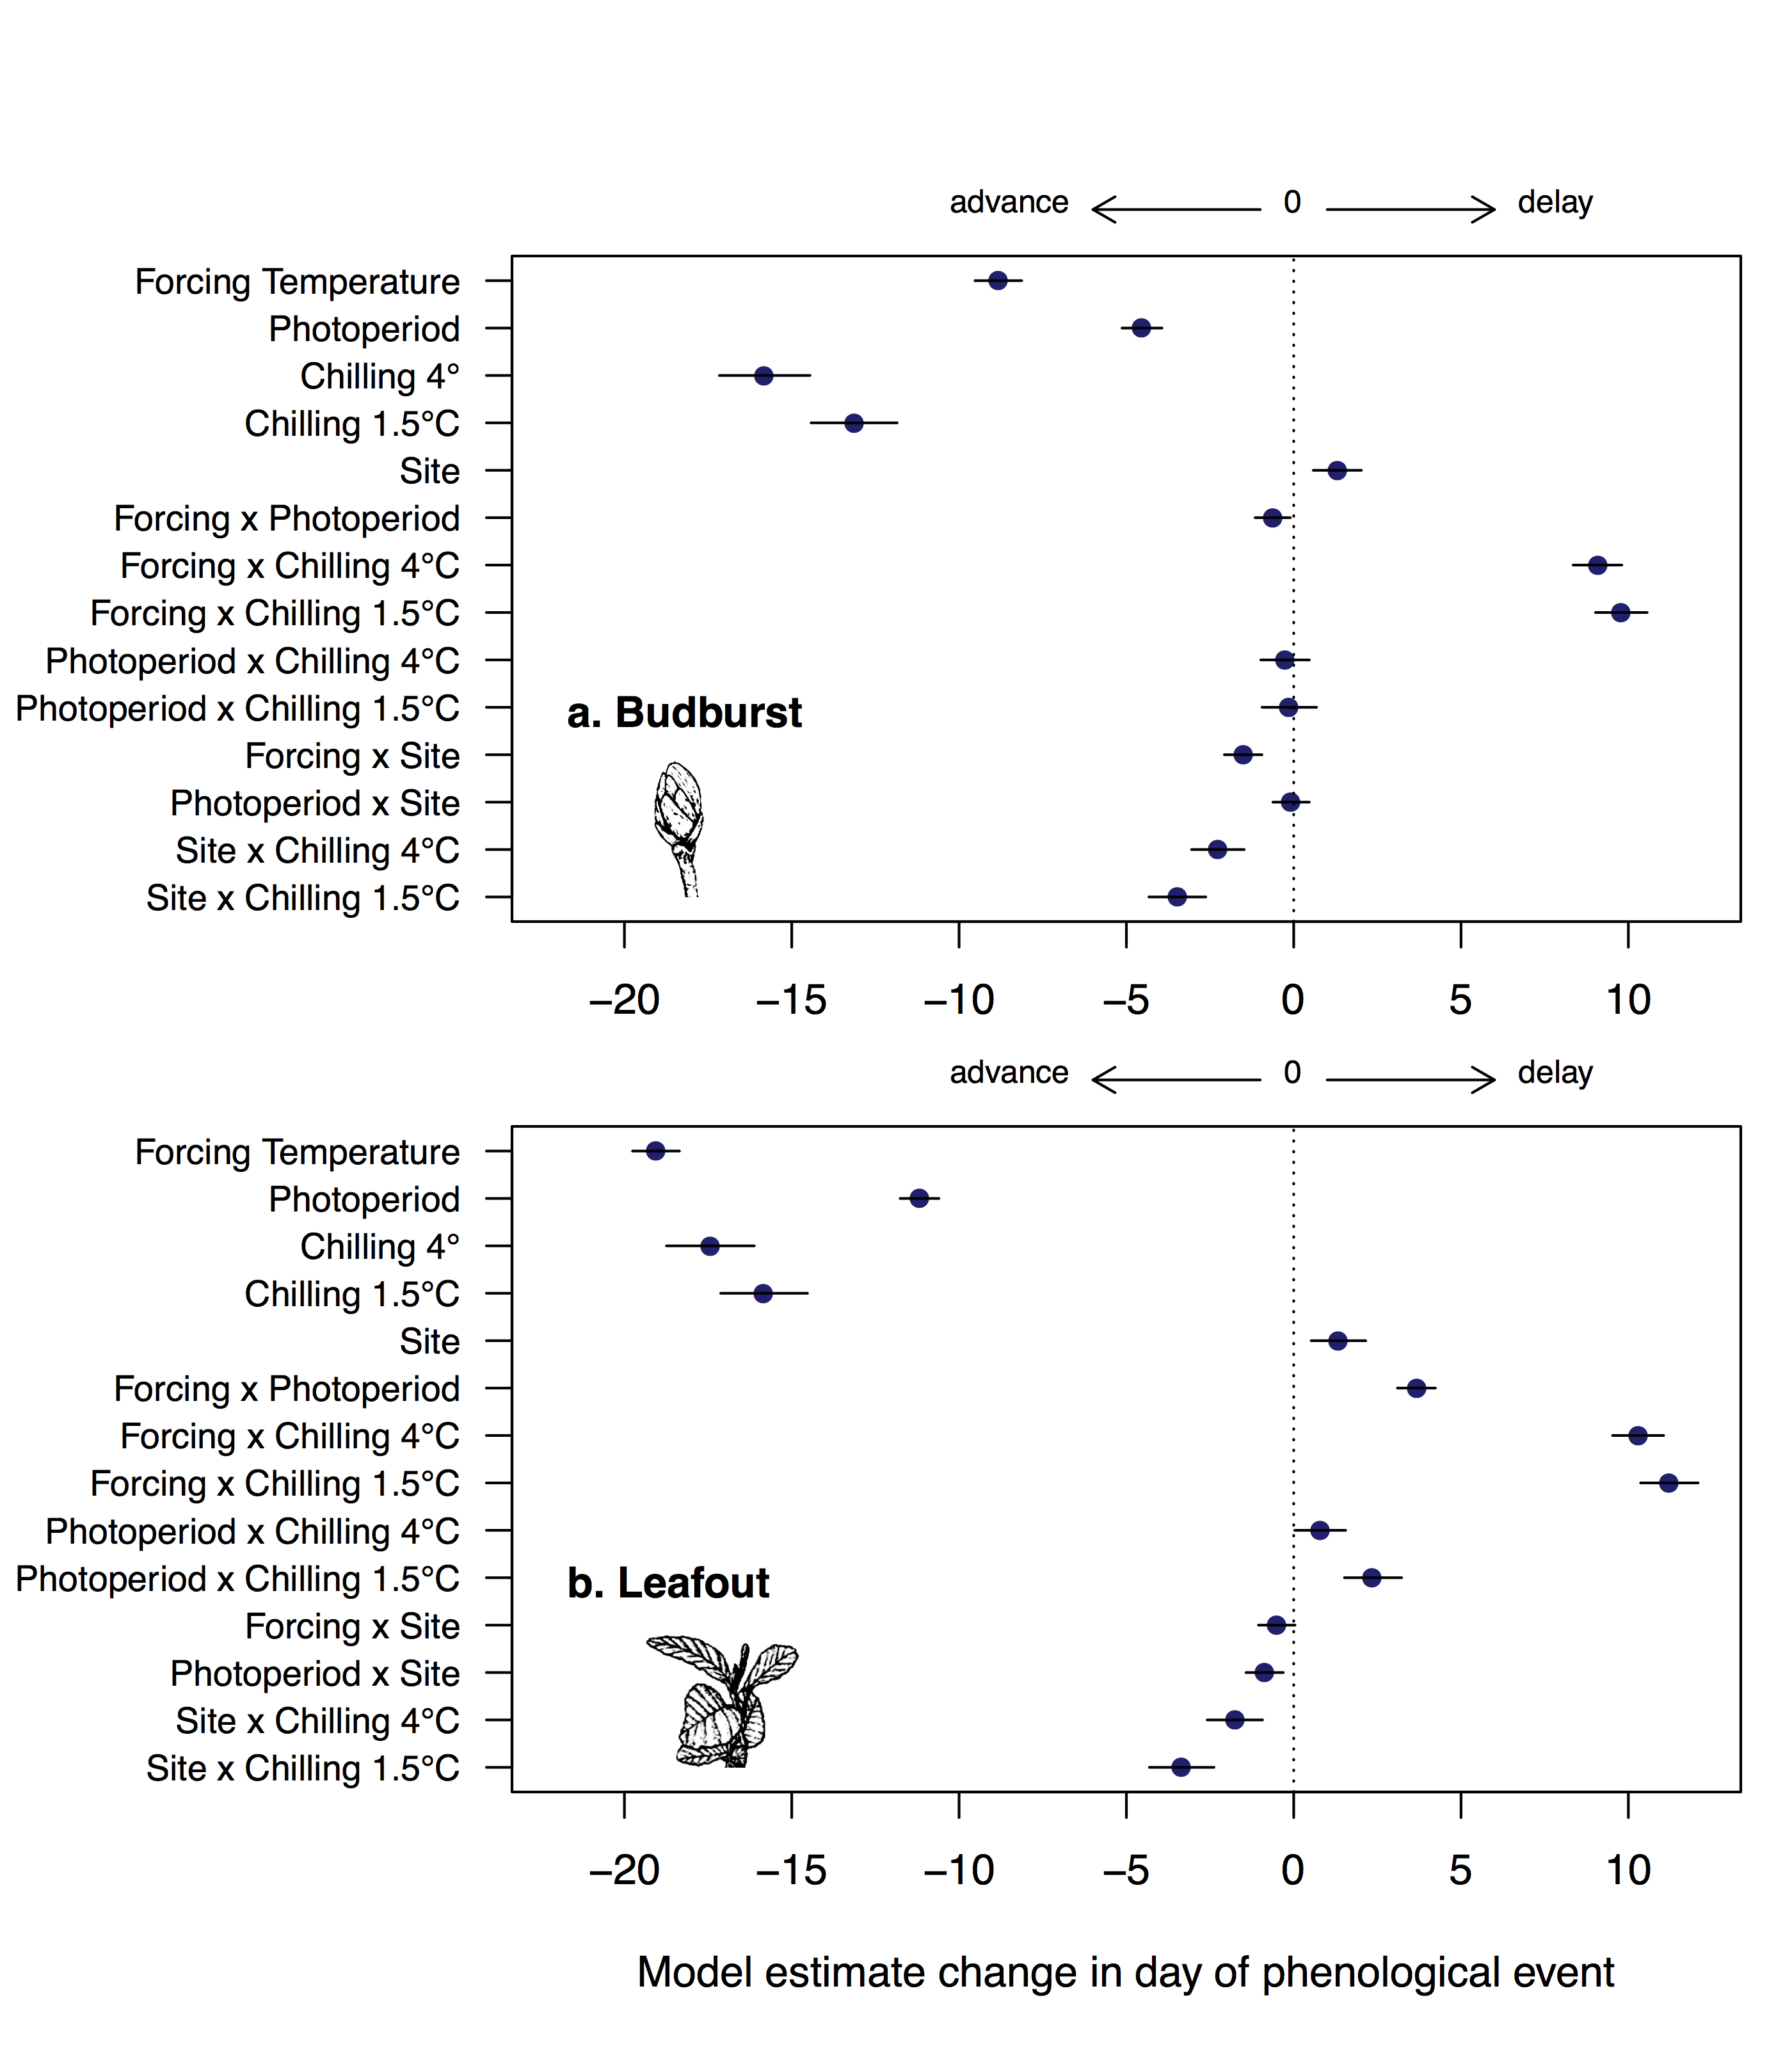
\includegraphics[width=0.9\textwidth]{images/Fig1_bb_lo.png}
\caption{Effects of forcing temperature, photoperiod, chilling and site on budburst (a) and leafout (b) days across 28 species. Dots and bars show mean and 50\% credible intervals from a Bayesian hierarchical model that also incorporated species-level variations (see Tables S5-S6; Figs. 1, S4-S5). Advances in phenology are shown by negative numbers; delays are shown as positive. Forcing temperatures and photoperiods were two levels each (see the Materials and Methods section), and chilling treatments were applied for 30 days. Budburst and leafout images from \citet{Finn:2007}.}
\label{fig:maineff}
\end{figure}

\newpage
\begin{figure}[h!]
\centering
%\noindent 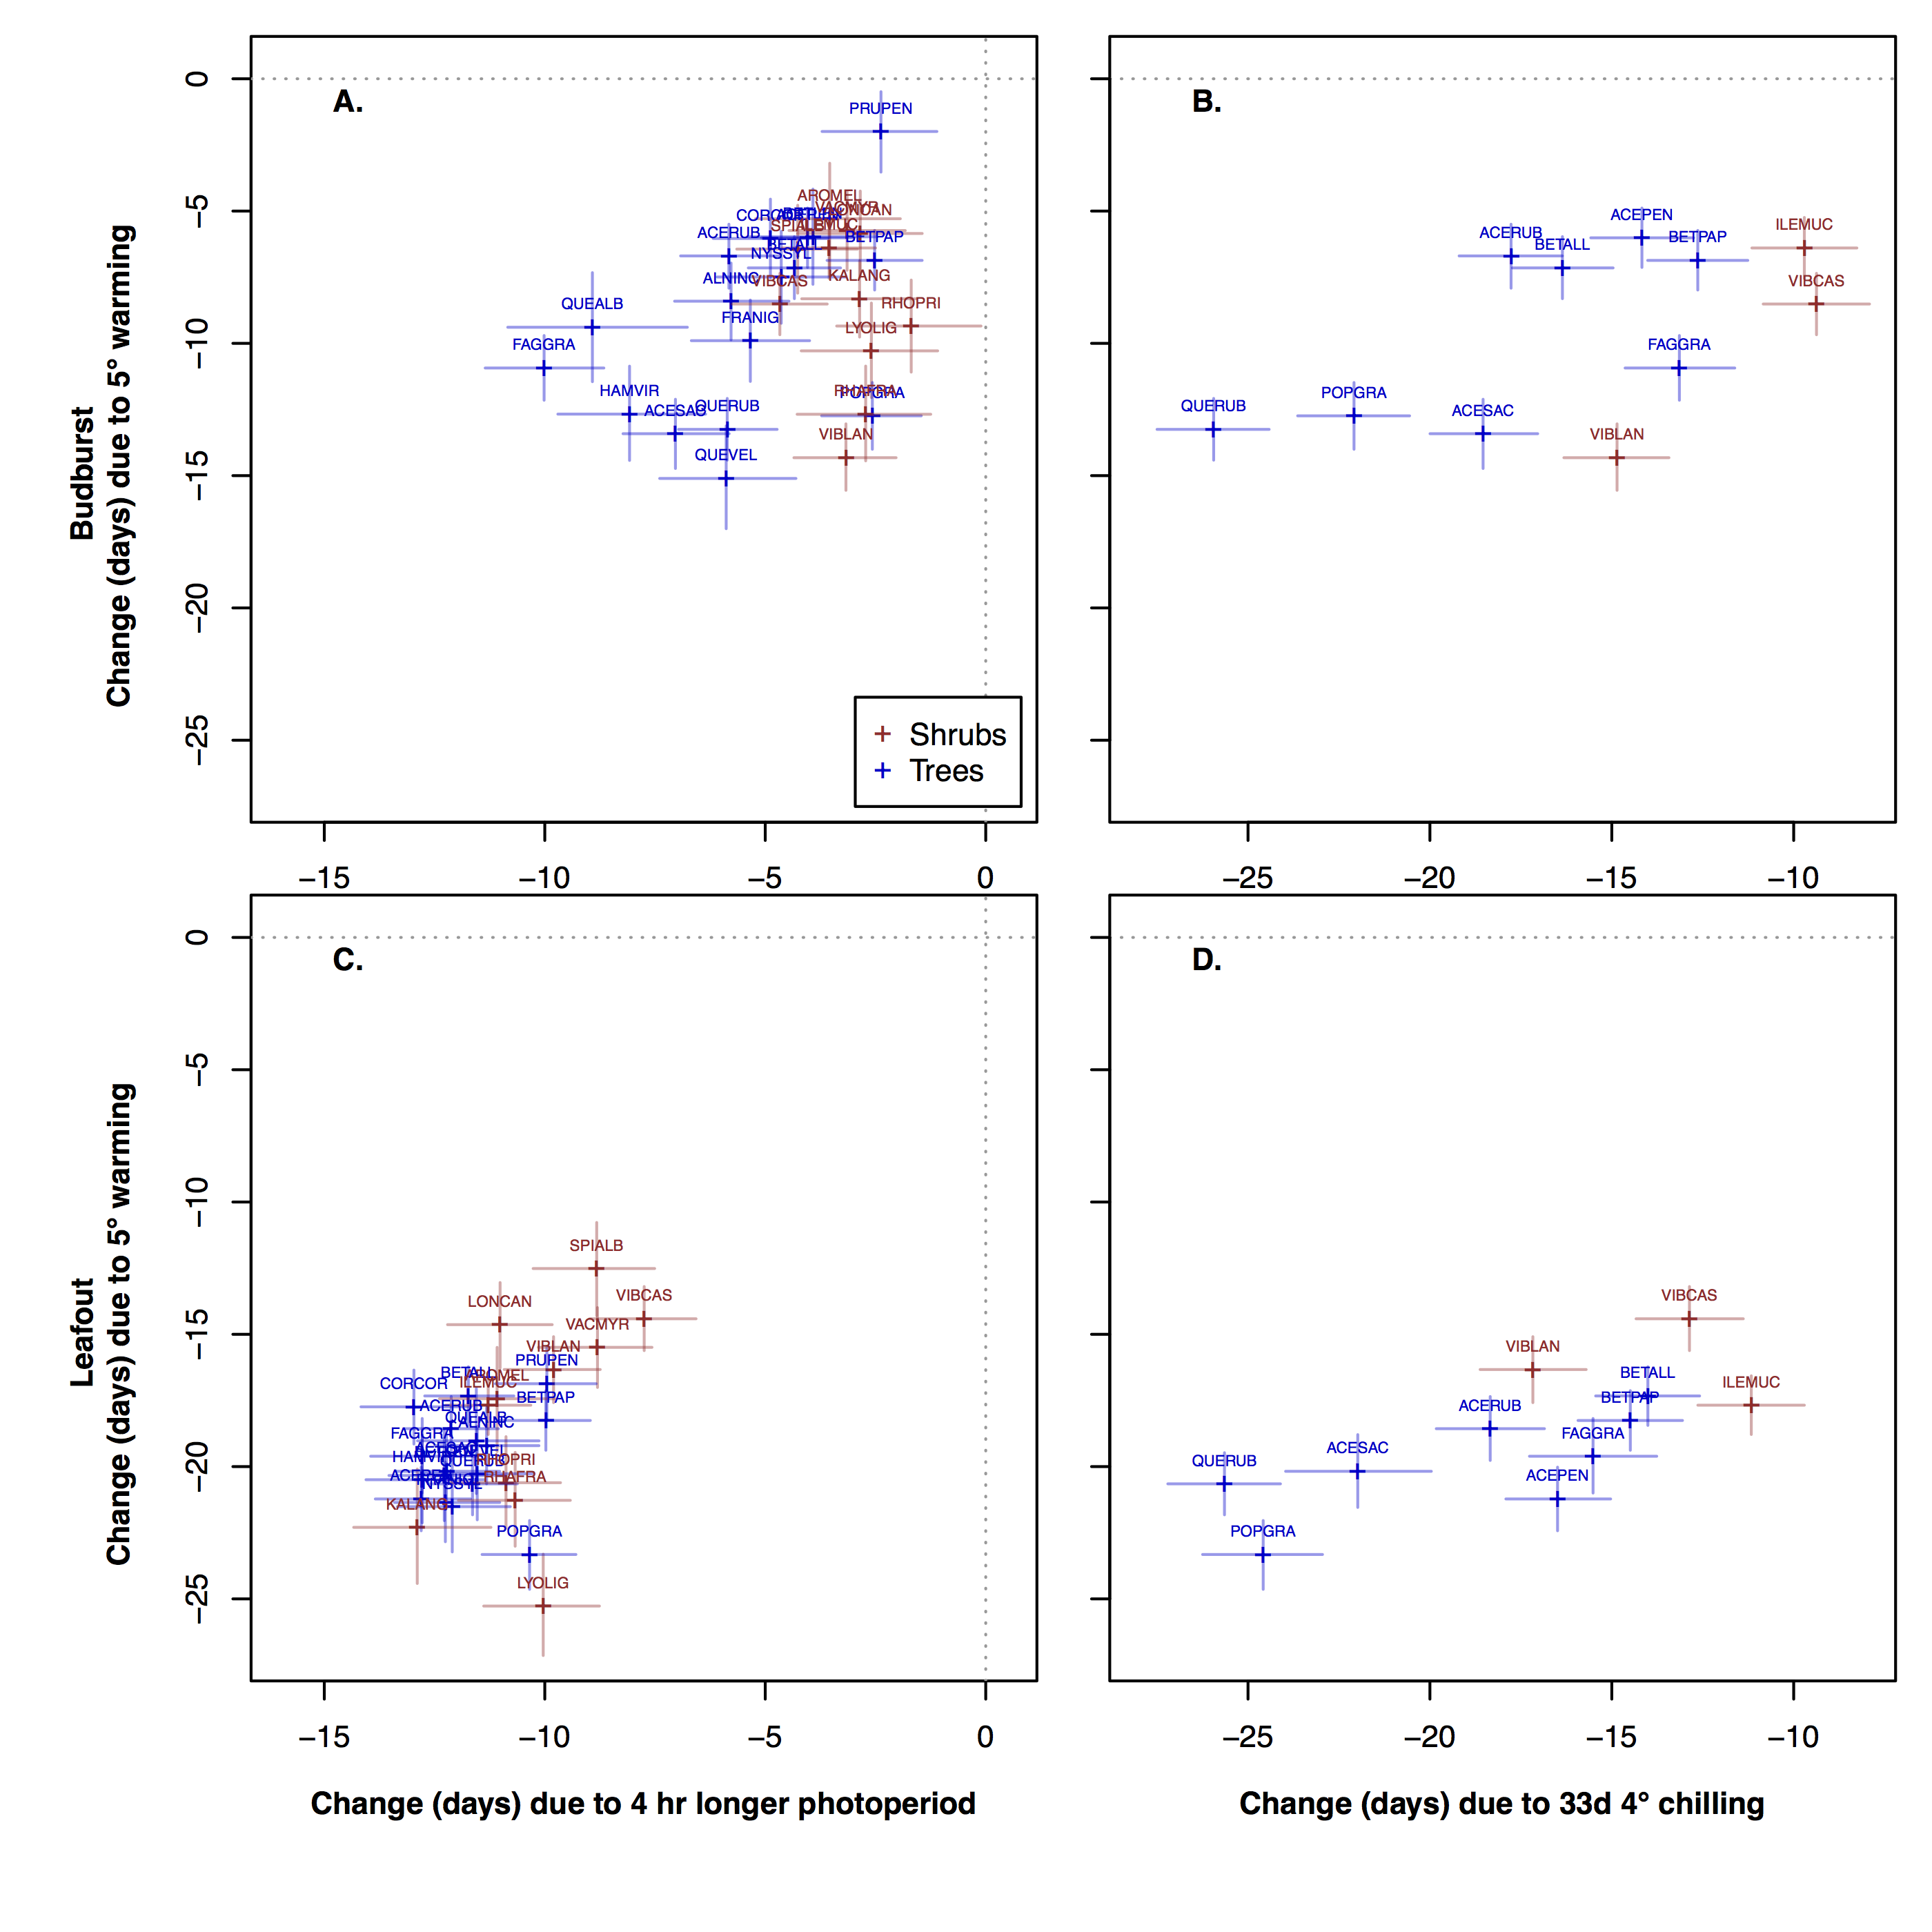
\includegraphics[width=1\textwidth]{images/Fig2_4panel.png}
\caption{Effects of warming on budburst day (A-B) and leafout day (C-D) compared to photoperiod (A, C) and chilling (B, D) across species (shrub species shown in red, tree species in blue): Crosses and bars show mean and 50\% credible intervals from a Bayesian hierarchical model (see Tables S5-S6; Figs. 1, S4-S5). For visualization purposes, species names are represented by the first three letters of the genus and first three letters of the species epithet (see Table S1 for full species names and Fig. S6-S8 for additional versions of figure).}
\label{fig:sppeff}
\end{figure}

\newpage
\begin{figure}
%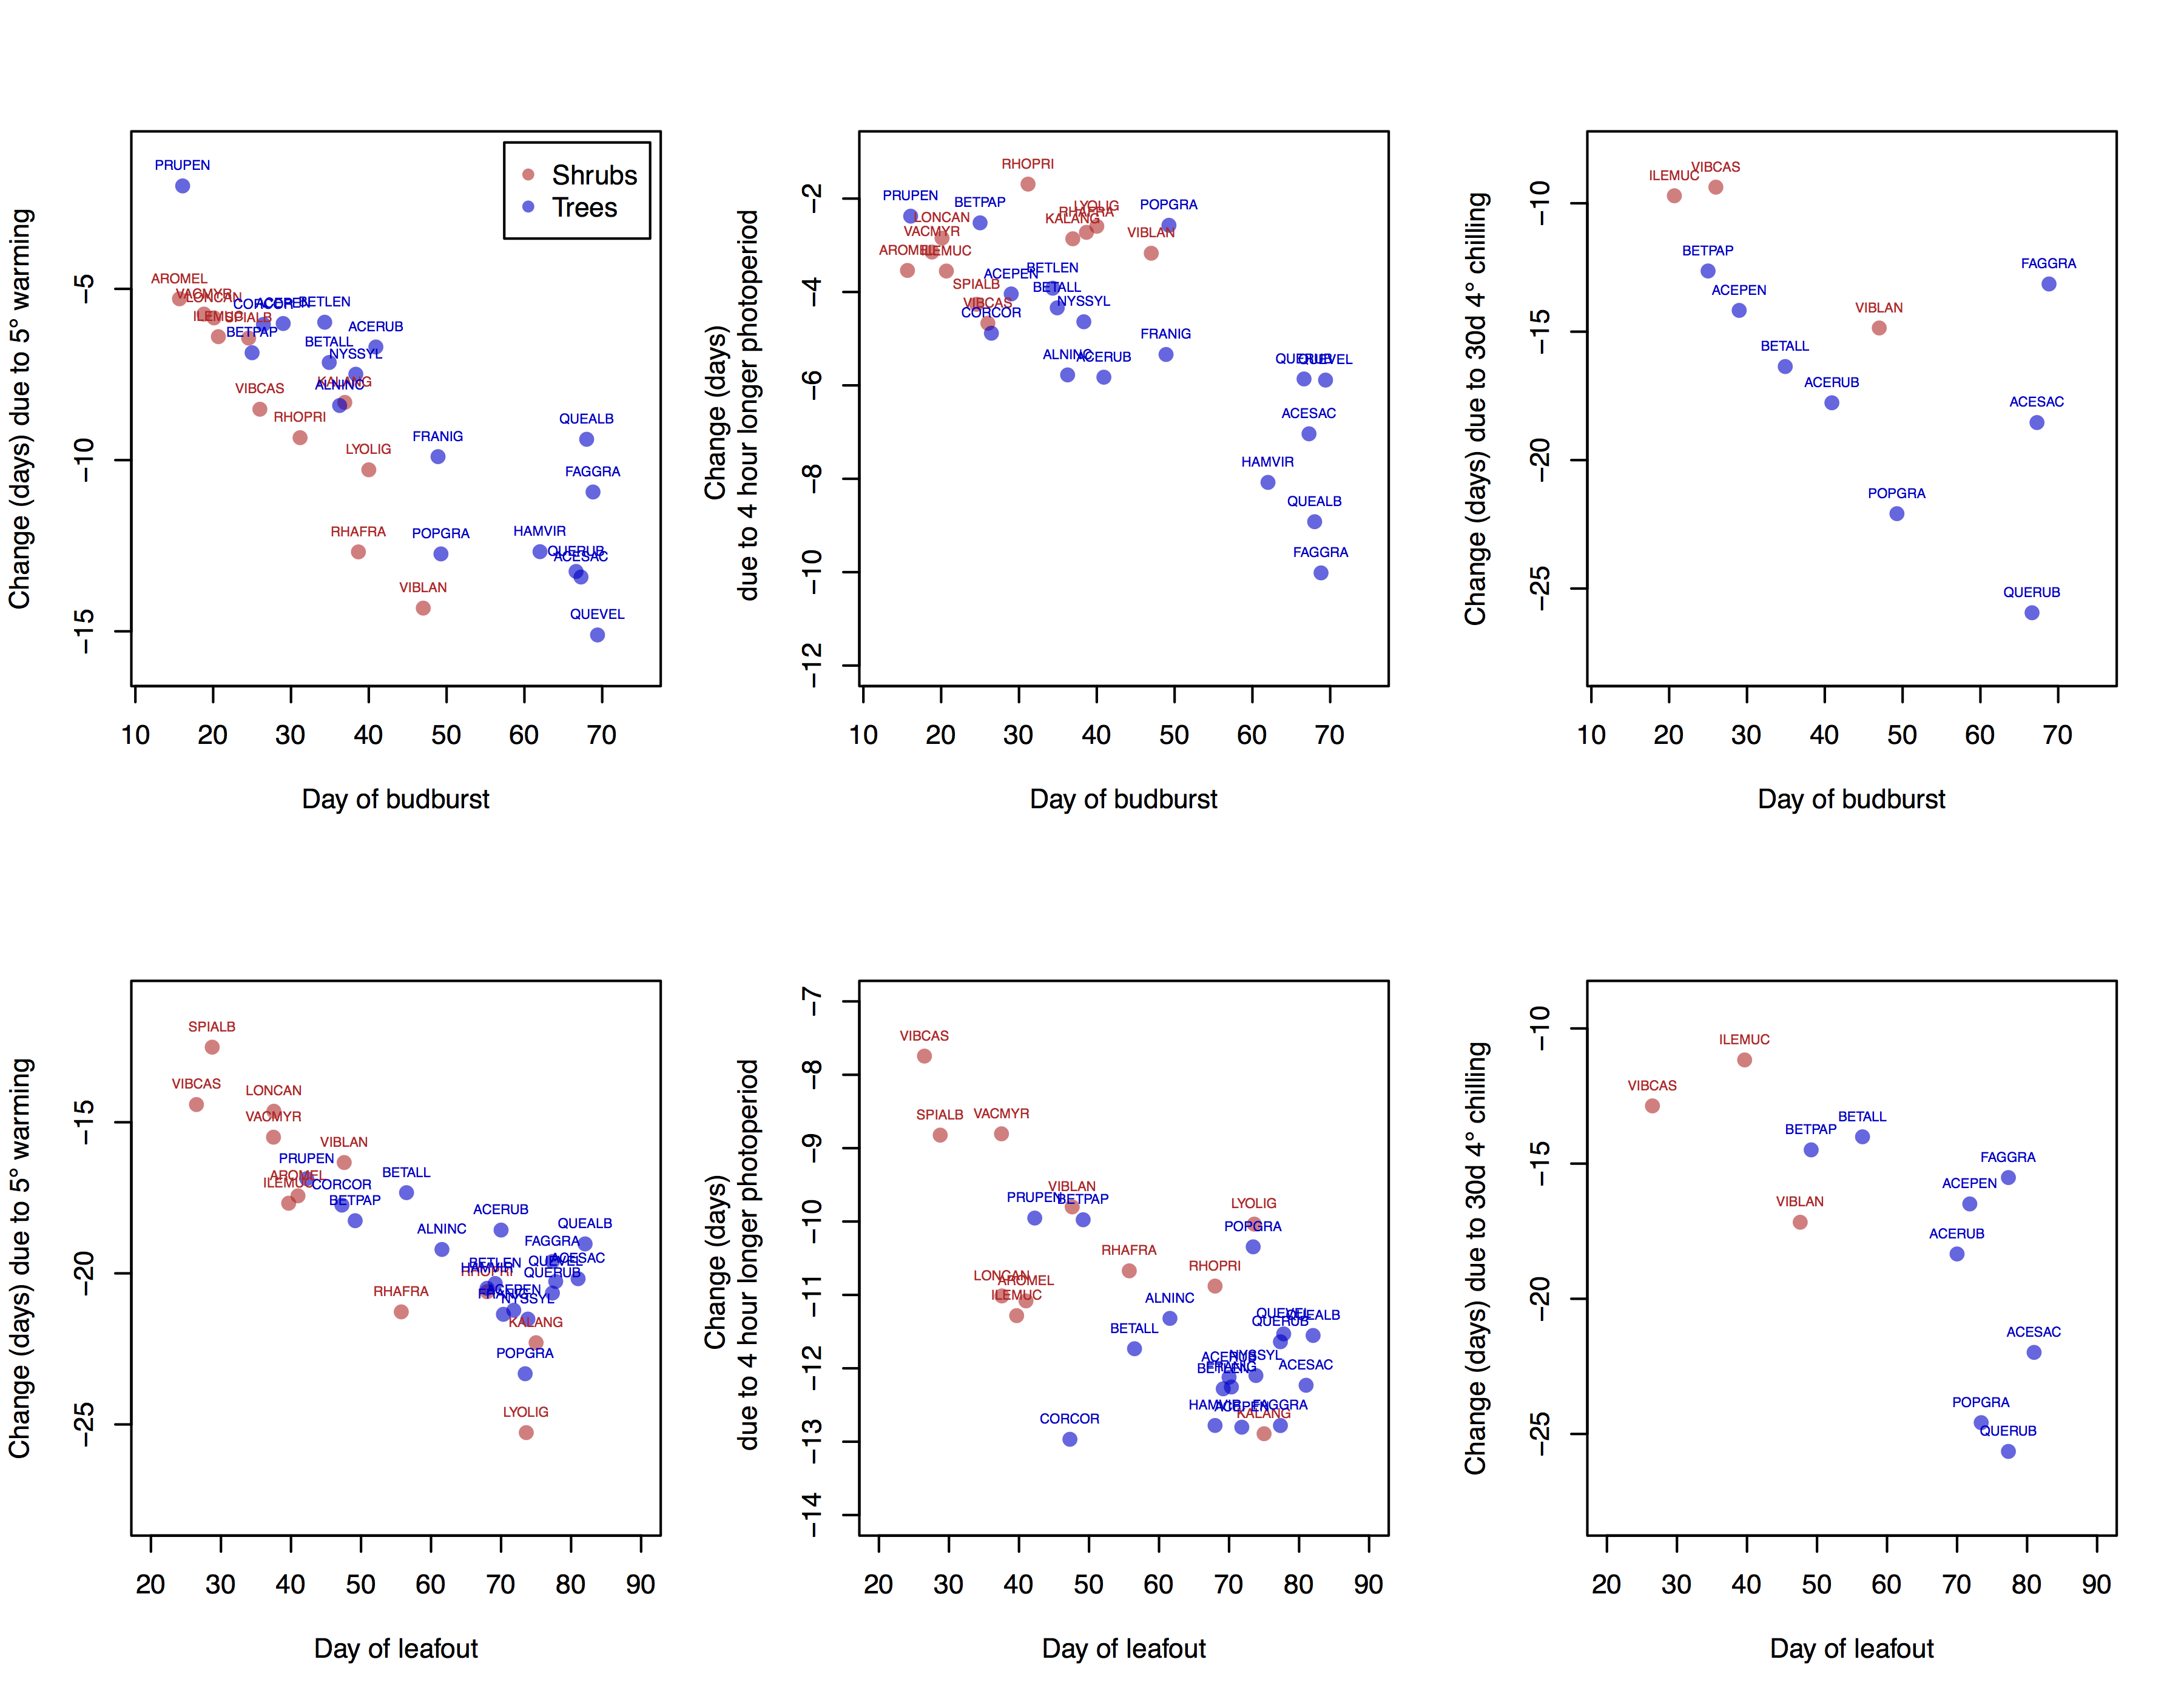
\includegraphics[width=1\textwidth]{Sens_vs_day_treeshrub.png}
\caption{Effects of photoperiod, temperature and chilling across species (shrub species shown in red, tree species in blue) compared to day of budburst (upper panels) or leafout (lower panels): we show mean estimates of sensitivity to warming, photoperiod, and chilling from a Bayesian hierarchical model (see Tables S5-S6; Figs. 1, S4-S5). For visualization purposes, species names are represented by the first three letters of the genus and first three letters of the species epithet (see Table S1 for full species names).}
\label{fig:commsens}
\end{figure}


\end{document}